\documentclass[aspectratio=169,10pt]{beamer}
\usetheme{Madrid}
\usecolortheme{default}
\usepackage{amsmath,amssymb,graphicx,booktabs,xcolor}
\usepackage{tikz}
\usetikzlibrary{arrows.meta,positioning,shapes.geometric}
\graphicspath{{figures/slides/}{figures/sim/}{figures/nb/}}
\setbeamertemplate{navigation symbols}{}

% ---------------------------------------------------------------------------
% Status markers -- search for PLACEHOLDER / PRELIMINARY / TBD before the talk
% ---------------------------------------------------------------------------
\newcommand{\placeholder}[1]{%
  \fcolorbox{red}{red!6}{\parbox{0.92\linewidth}{\color{red!70!black}\footnotesize\textbf{PLACEHOLDER:} #1}}}
\newcommand{\figph}[2]{%
  \fcolorbox{red}{red!6}{\parbox[c][#1][c]{0.92\linewidth}{\centering\color{red!70!black}\footnotesize
  \textbf{FIGURE PLACEHOLDER}\\[2pt] #2}}}
\newcommand{\prelim}{\textcolor{orange!90!black}{\textbf{[PRELIMINARY]}}}
\newcommand{\tbd}{\textcolor{red!70!black}{\textbf{TBD}}}
\newcommand{\src}[1]{\par\vfill\hfill{\tiny\color{gray}#1}}
% numbers (and figures) still from the first campaign: +-300 / +-500 nm and +-5 um;
% the rerun at +-lambda/2 and +-8 lambda replaces them -- remove the marks then
\newcommand{\oldrange}{\textcolor{orange!90!black}{\textbf{[old ranges]}}}
\newcommand{\oldnote}{\par\vfill{\tiny\color{orange!90!black}\textbf{[old ranges]} numbers and plots
  from the first campaign ($\pm300$ / $\pm500$ nm single, $\pm5\,\mu$m spectral); the rerun at
  $\pm\lambda/2$ and $\pm8\lambda$ is running and replaces them.}}

\title[Piston sensing with a dispersed photonic lantern]{Piston Sensing with a Dispersed Photonic Lantern}
\subtitle{From how a lantern works to a 7- vs 19-port study for ANDES \\ \footnotesize(work in progress -- placeholders marked in red)}
\author{Fabio Rossi}
\institute{INAF -- Osservatorio Astrofisico di Arcetri}
\date{\tbd}

\begin{document}

\begin{frame}
\titlepage
\end{frame}

\begin{frame}{Outline}
\tableofcontents[hideallsubsections]
\end{frame}

% ===========================================================================
\section{What a photonic lantern is and how it works}
% ===========================================================================
\begin{frame}{The problem: limits of pupil-plane sensors}
\begin{itemize}
    \item Shack-Hartmann and pyramid sensors work in or near a pupil plane and measure local
          gradients of the wavefront phase: large dynamic range, well understood.
    \item Three problems dominate once the atmosphere is already well corrected:
    \begin{enumerate}
        \item \textbf{Non-common-path aberrations}: invisible to a separate sensing arm.
        \item \textbf{Petal / island modes}: piston steps between pupil fragments have (almost)
              zero gradient where the light is; finite spiders give only a weak edge-diffraction signal.
        \item \textbf{Photon loss}: light diverted to the sensor is lost to science.
    \end{enumerate}
    \item A \textbf{focal-plane} sensor sees all three -- if it can measure phase, not just intensity.
\end{itemize}
\end{frame}

\begin{frame}{The photonic lantern: a focal-plane wavefront sensor}
\begin{columns}[T]
\begin{column}{0.55\textwidth}
\begin{itemize}
    \item A slowly tapered fibre device: \textbf{one few-mode end} $\leftrightarrow$
          \textbf{$N$ single-mode cores}.
    \item Placed at the \textbf{science focus}: no non-common path.
    \item Its $N$ guided modes \textbf{interfere with fixed, device-specific phases}
          on the way to the cores $\Rightarrow$ the core intensities encode the focal-plane
          \emph{phase}, including the sign of even aberrations.
    \item Outputs are single-mode fibres: the same photons can feed a spectrograph.
    \item \textbf{Price}: low order ($\lesssim N$ modes), modest range, device-specific
          response that must be calibrated or simulated.
\end{itemize}
\end{column}
\begin{column}{0.43\textwidth}
\centering
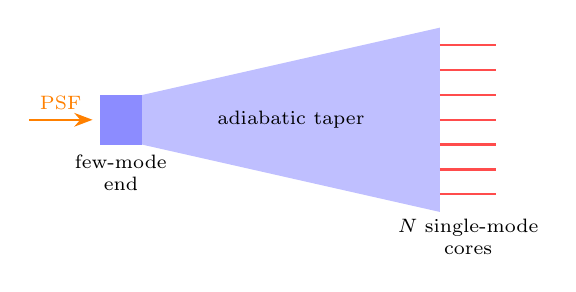
\begin{tikzpicture}[scale=0.9]
  \fill[blue!25] (0,0.35) -- (4.2,1.3) -- (4.2,-1.3) -- (0,-0.35) -- cycle;
  \fill[blue!45] (-0.6,0.35) rectangle (0,-0.35);
  \foreach \y in {-1.05,-0.7,-0.35,0,0.35,0.7,1.05} {\draw[red!70, thick] (4.2,\y) -- (5.0,\y);}
  \node[align=center, font=\scriptsize] at (-0.3,-0.75) {few-mode\\end};
  \node[align=center, font=\scriptsize] at (4.6,-1.65) {$N$ single-mode\\cores};
  \node[font=\scriptsize] at (2.1,0) {adiabatic taper};
  \draw[-{Stealth}, thick, orange] (-1.6,0) -- (-0.7,0) node[midway, above, font=\scriptsize] {PSF};
\end{tikzpicture}
\end{column}
\end{columns}
\end{frame}

\begin{frame}{Guided (bound) modes and the effective index}
\begin{columns}[T]
\begin{column}{0.52\textwidth}
\small
\begin{itemize}
    \item A \textbf{mode} is a transverse field pattern that propagates without changing its shape:
          $E(x,y,z) = \psi(x,y)\,e^{i\beta z}$, with
          $\nabla_\perp^2 \psi + k_0^2 n^2(x,y)\,\psi = \beta^2 \psi$, \ $k_0 = 2\pi/\lambda$.
    \item A \textbf{bound (guided) mode} keeps its power in and around the core: its field decays
          exponentially in the cladding, so it travels along the fibre without radiating.
          Patterns that are not bound leak their power sideways (radiation modes) within a short distance.
    \item \textbf{Effective index} $n_\mathrm{eff} = \beta/k_0$: the mode's phase advances along $z$
          as for a plane wave in a uniform medium of index $n_\mathrm{eff}$. It is a weighted average
          of the indices the mode sees: bound modes have $n_2 < n_\mathrm{eff} < n_1$; well-confined
          (low-order) modes are close to $n_1$, modes near cut-off close to $n_2$.
\end{itemize}
\end{column}
\begin{column}{0.47\textwidth}
\centering
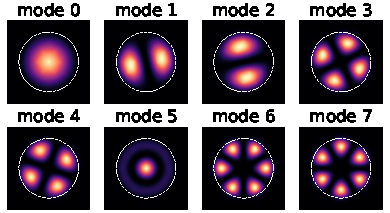
\includegraphics{pl19_800_modes_input}\\
{\scriptsize The first 8 bound modes at the multimode end of the 19-port lantern, in
decreasing $n_\mathrm{eff}$ (cbeam simulation, 800 nm).}
\end{column}
\end{columns}
\end{frame}

\begin{frame}{Numerical aperture and the number of bound modes}
\begin{columns}[T]
\begin{column}{0.52\textwidth}
\small
\begin{itemize}
    \item Core index $n_1$, cladding index $n_2 < n_1$. A ray is trapped by total internal
          reflection if it enters within the acceptance angle $\theta_\mathrm{max}$:
          \[ \mathrm{NA} = n_0 \sin\theta_\mathrm{max} = \sqrt{n_1^2 - n_2^2} \]
          ($n_0 = 1$ outside the fibre).
    \item The number of bound modes is set by the normalised frequency
          \[ V = \frac{2\pi a}{\lambda}\,\mathrm{NA}, \qquad N_\mathrm{modes} \approx V^2/4 \]
          ($a$: core radius). Single-mode if $V < 2.405$.
    \item A lantern needs $\approx N$ bound modes at its multimode end. There the role of $n_1$ is
          played by the cladding and that of $n_2$ by the low-index jacket.
\end{itemize}
\end{column}
\begin{column}{0.46\textwidth}
\centering
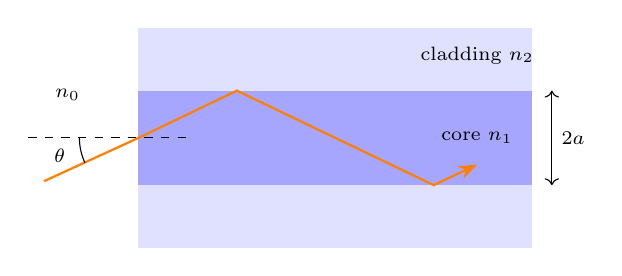
\begin{tikzpicture}[scale=1.0]
  \fill[blue!12] (0,-1.4) rectangle (5,1.4);
  \fill[blue!35] (0,-0.6) rectangle (5,0.6);
  \node[font=\scriptsize] at (4.3,1.05) {cladding $n_2$};
  \node[font=\scriptsize] at (4.3,0.0) {core $n_1$};
  \draw[thick, orange, -{Stealth}] (-1.2,-0.55) -- (0,0) -- (1.25,0.6) -- (2.5,0) -- (3.75,-0.6) -- (4.3,-0.34);
  \draw[dashed] (-1.4,0) -- (0.6,0);
  \draw (-0.75,0) arc (180:205:0.75);
  \node[font=\scriptsize] at (-1.0,-0.23) {$\theta$};
  \node[font=\scriptsize, align=center] at (-0.9,0.55) {$n_0$};
  \draw[<->] (5.25,-0.6) -- (5.25,0.6) node[midway, right, font=\scriptsize] {$2a$};
\end{tikzpicture}\\[4pt]
{\scriptsize rays entering within $\theta \le \theta_\mathrm{max}$ are guided}
\end{column}
\end{columns}
\end{frame}

\begin{frame}{A concrete lantern: the 19-port, 800 nm reference design}
\centering
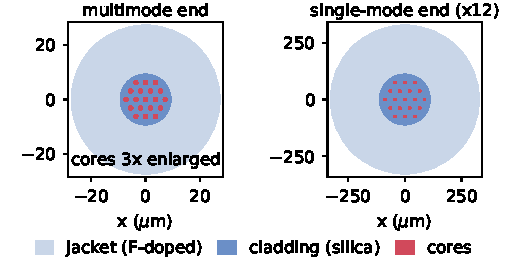
\includegraphics{pl19_800_geometry}
\begin{itemize}\small
    \item Cladding (silica, $n=1.444$) inside a low-index jacket ($\Delta n = -5.5\times10^{-3}$):
          at the waist the cladding \emph{is} the multimode core ($V = 8.9$, $\sim$23 bound modes).
    \item 19 cores ($\Delta n = +8.8\times10^{-3}$), tapered $\times 12$ over 100 mm.
\end{itemize}
\src{cbeam (J.~Lin) -- \texttt{batch\_pipeline} preset \texttt{pl19\_800}}
\end{frame}

\begin{frame}{Supermodes}
\begin{columns}[T]
\begin{column}{0.55\textwidth}
\small
\begin{itemize}
    \item A \textbf{supermode} is a bound mode of the \emph{whole} cross-section -- all cores,
          cladding and jacket together -- not of a single core.
    \item Two identical cores close together: their individual modes overlap and couple; the
          bound modes of the pair are the symmetric and antisymmetric combinations, with
          slightly different $n_\mathrm{eff}$. With $N$ cores: $N$ supermodes.
    \item Light launched into one core beats between the supermodes: this is how power moves
          from core to core (the directional coupler).
    \item In a lantern the supermodes change along $z$:
    \begin{itemize}
        \item waist: cores too small to guide $\Rightarrow$ supermodes $=$ LP modes of the cladding guide;
        \item single-mode end: cores far apart $\Rightarrow$ $N$ degenerate supermodes $\approx$ the individual core modes.
    \end{itemize}
\end{itemize}
\end{column}
\begin{column}{0.44\textwidth}
\centering
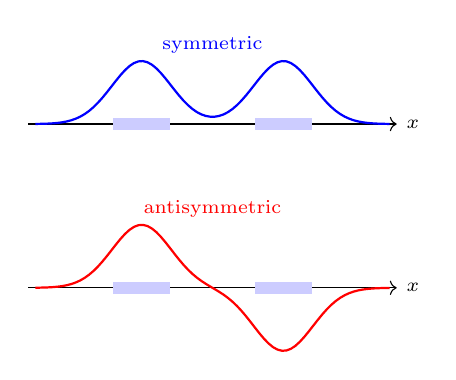
\begin{tikzpicture}[xscale=0.9, yscale=0.8]
  \draw[->] (-2.6,0) -- (2.6,0) node[right, font=\scriptsize] {$x$};
  \fill[blue!20] (-1.4,-0.1) rectangle (-0.6,0.1); \fill[blue!20] (0.6,-0.1) rectangle (1.4,0.1);
  \draw[thick, blue, domain=-2.5:2.5, samples=80] plot (\x, {exp(-(\x+1)^2/0.35)+exp(-(\x-1)^2/0.35)});
  \node[font=\scriptsize, blue] at (0,1.25) {symmetric};
  \begin{scope}[yshift=-2.6cm]
  \draw[->] (-2.6,0) -- (2.6,0) node[right, font=\scriptsize] {$x$};
  \fill[blue!20] (-1.4,-0.1) rectangle (-0.6,0.1); \fill[blue!20] (0.6,-0.1) rectangle (1.4,0.1);
  \draw[thick, red, domain=-2.5:2.5, samples=80] plot (\x, {exp(-(\x+1)^2/0.35)-exp(-(\x-1)^2/0.35)});
  \node[font=\scriptsize, red] at (0,1.25) {antisymmetric};
  \end{scope}
\end{tikzpicture}\\
{\scriptsize the two supermodes of two coupled cores (field)}
\end{column}
\end{columns}
\end{frame}

\begin{frame}{Inside the taper: from LP modes to core modes}
\begin{columns}[T]
\begin{column}{0.62\textwidth}
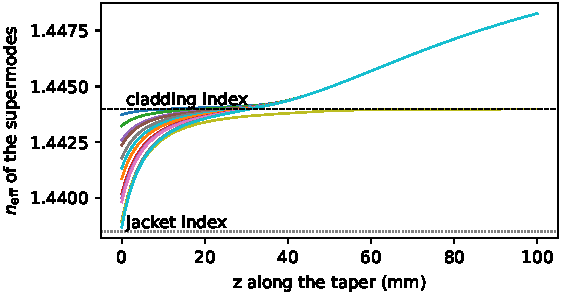
\includegraphics{pl19_800_neff_vs_z}
\end{column}
\begin{column}{0.37\textwidth}
\small
\begin{itemize}
    \item Multimode end ($z=0$): cores too small to guide; the supermodes are the LP modes of
          the cladding guide, well separated in $n_\mathrm{eff}$.
    \item Along the taper the cores grow and capture the light; the supermodes merge.
    \item Single-mode end: 19 \textbf{degenerate} core modes (+ one cladding mode, lost).
    \item Adiabatic: each supermode follows its own curve, \textbf{no power exchange}
          -- but each picks up its own phase $\int\beta\,dz$.
\end{itemize}
\end{column}
\end{columns}
\end{frame}

\begin{frame}{How we simulate it (1): characterizing the lantern}
\small
cbeam (J.~Lin) solves the scalar, paraxial problem with \textbf{coupled-mode theory}: the field
is written on the local supermodes $\xi_n(x,y;z)$ of the cross-section at each $z$,
\[ u(x,y,z) = \sum_{n=1}^{N} a_n(z)\,\xi_n(x,y;z). \]
Characterization (once per lantern and wavelength), along an adaptive grid of $z$ values:
\begin{enumerate}
    \item \textbf{Eigen-solve} the cross-section at $z$ with finite elements (mesh scaled by the
          local taper factor): $\nabla_\perp^2 \xi_n + k_0^2 n^2(x,y;z)\,\xi_n = \beta_n^2 \xi_n$
          $\Rightarrow$ $\beta_n(z)$, $\xi_n(z)$ for the $N$ tracked modes.
    \item \textbf{Track} the modes from one $z$ to the next: match them by overlap, fix their sign,
          align the bases of degenerate pairs; the step shrinks where the modes change fast.
    \item \textbf{Couplings} $\kappa_{mn}(z) = \langle \xi_m | \partial_z \xi_n \rangle$ from the
          $z$-derivative of the spline-interpolated modes (corrected for the moving mesh);
          $\kappa$ is antisymmetric.
\end{enumerate}
Cost: $\sim$1--2 min per wavelength (7 ports) to $\sim$13 min (19 ports); cached and reused.
\end{frame}

\begin{frame}{How we simulate it (2): propagating fields}
\begin{columns}[T]
\begin{column}{0.56\textwidth}
\small
\begin{itemize}
    \item Substituting the expansion in the paraxial equation and projecting on $\xi_m$ gives a
          \textbf{linear ODE for the $N$ amplitudes}. Removing each mode's own fast phase,
          $a_n = c_n\,e^{i\Theta_n}$ with $\Theta_n(z) = \int_0^z \beta_n\,dz'$:
          \[ \frac{dc_m}{dz} = -\sum_n \kappa_{mn}(z)\,e^{\,i[\Theta_n(z) - \Theta_m(z)]}\,c_n \]
    \item Integrated from $z=0$ to $L$ with an adaptive Runge-Kutta solver (tolerance
          $10^{-12}$), for thousands of input fields at once (one batched call).
    \item Adiabatic limit ($|\kappa_{mn}| \ll |\beta_n - \beta_m|$): the $c_n$ stay constant --
          each supermode keeps its power and only accumulates its phase $\Theta_n(L)$.
    \item At $z = L$: project the supermodes on the individual core modes $\Rightarrow$ the core
          amplitudes $v_k$.
\end{itemize}
\end{column}
\begin{column}{0.42\textwidth}
\centering
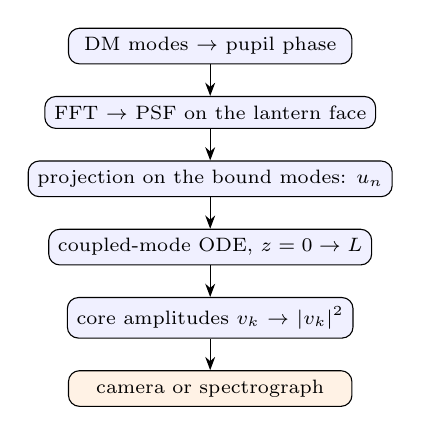
\begin{tikzpicture}[node distance=0.4cm, every node/.style={font=\scriptsize, draw, rounded corners,
                    fill=blue!6, minimum width=3.6cm, align=center}]
  \node (a) {DM modes $\to$ pupil phase};
  \node (b) [below=of a] {FFT $\to$ PSF on the lantern face};
  \node (c) [below=of b] {projection on the bound modes: $u_n$};
  \node (d) [below=of c] {coupled-mode ODE, $z = 0 \to L$};
  \node (e) [below=of d] {core amplitudes $v_k$ $\to$ $|v_k|^2$};
  \node (f) [below=of e, fill=orange!10] {camera or spectrograph};
  \foreach \x/\y in {a/b,b/c,c/d,d/e,e/f} \draw[-{Stealth}] (\x) -- (\y);
\end{tikzpicture}
\end{column}
\end{columns}
\src{50\,000 fields $\times$ 41 wavelengths: $\sim$1.5 h on 50 cores within half of the server's memory}
\end{frame}

\begin{frame}{The lantern as a matrix: $\mathbf v = A\,\mathbf u$}
\begin{columns}[T]
\begin{column}{0.64\textwidth}
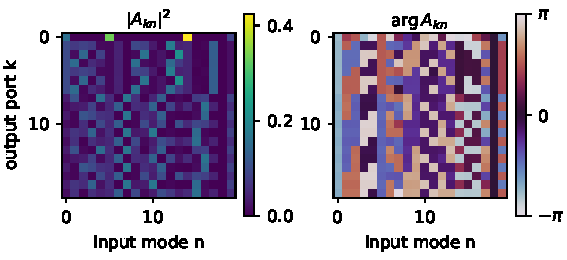
\includegraphics{pl19_800_transfer_matrix}
\end{column}
\begin{column}{0.35\textwidth}
\small
\begin{itemize}
    \item Column $n$: launch multimode mode $n$ alone, read the 19 cores.
    \item Each input mode illuminates many cores; the \textbf{phases} of $A$ are what make
          the lantern a wavefront sensor.
    \item Unitary on the guided subspace (lossless, adiabatic lantern).
    \item Depends on wavelength, temperature, fabrication: measured or simulated, per device.
\end{itemize}
\end{column}
\end{columns}
\end{frame}

\begin{frame}{The transfer matrix in detail}
\small
\begin{itemize}
    \item Definition: $A_{kn} = \langle \phi_k \,|\, \mathcal U(L)\,\psi_n \rangle$ -- launch bound mode
          $\psi_n$ of the multimode end, propagate ($\mathcal U$: the coupled-mode solution), project on the
          mode $\phi_k$ of output core $k$. Computed by propagating each unit vector $\mathbf e_n$.
    \item Size: 19 cores $\times$ 20 tracked modes. Mode 18 does not reach any core (it ends as
          cladding light and is dropped): its column is empty.
    \item \textbf{Unitary} on the 19 guided modes to within 0.7\% here: $\sum_k |A_{kn}|^2 = 0.993$--$0.997$
          (the rest is numerical; real losses would show as smaller column norms).
    \item \textbf{Phases}: a phase per row is unobservable (we detect $|v_k|^2$); the column phases follow
          the sign convention of the modes used to compute $u_n$ and must be consistent with it.
    \item \textbf{Structure}: the central core is fed mostly by the radially symmetric modes 14 and 5
          (42\% and 33\% of $|A_{0n}|^2$); degenerate partner modes give pairs of similar columns.
    \item Depends on wavelength (one $A$ per wavelength: 41 here), temperature and fabrication:
          every real lantern must be calibrated.
    \item With the projection written in the pupil, the whole sensor is one matrix:
          $\mathbf p = |A M \mathbf f|^2$, $\mathbf f$ = pupil field, $M$ = bound modes carried back to the pupil.
\end{itemize}
\end{frame}

\begin{frame}{Forward model: each output is an $N$-beam interferometer}
\begin{enumerate}
    \item Pupil field $P\,e^{i\varphi}$ $\to$ focal field $E = \mathcal F[P e^{i\varphi}]$.
    \item Projection on the guided modes: $u_n = \langle \psi_n | E \rangle$.
    \item Lantern: $\mathbf v = A\mathbf u$; detection $p_k = |v_k|^2$.
\end{enumerate}
\[
  p_k = \sum_n |A_{kn}|^2 |u_n|^2 + 2\sum_{n<n'} \mathrm{Re}\!\left[A_{kn}A_{kn'}^* u_n u_{n'}^*\right]
\]
\begin{itemize}
    \item The interference terms carry the phase information; the fixed phase offsets
          $\arg A_{kn} - \arg A_{kn'}$ let a standard lantern see \textbf{even} aberrations with sign
          (a camera, $A$ real, or a mode-selective lantern, $A$ diagonal, cannot).
    \item Only $N$ intensities per wavelength, normalised: $N-1$ independent numbers.
          \textbf{Keep this in mind for Part~4.}
\end{itemize}
\end{frame}

\begin{frame}{Example: one petal piston, seen by the lantern}
\begin{columns}[T]
\begin{column}{0.56\textwidth}
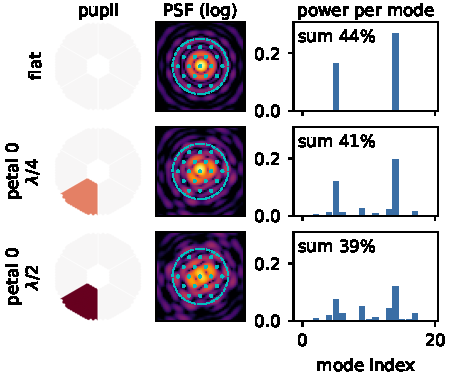
\includegraphics{pl19_800_psf_coupling}
\end{column}
\begin{column}{0.43\textwidth}
\small
\begin{itemize}
    \item Left to right: pupil (one petal pushed), PSF on the lantern face (dashed: multimode
          core; dots: cores), power in each guided mode.
    \item A petal piston reshapes the PSF and spreads light over many modes; the coupled
          fraction drops only slowly (44\% $\to$ 39\%).
    \item The first mode (LP$_{01}$) gets almost no light, even for a flat wavefront -- next slide.
    \item The coupled fraction ($\sim$44\%) reflects the PSF size choice of this design
          (see appendix).
\end{itemize}
\end{column}
\end{columns}
\end{frame}

\begin{frame}{Why does the first mode carry (almost) no light?}
\begin{columns}[T]
\begin{column}{0.45\textwidth}
\small
\begin{itemize}
    \item The coupling is an overlap, and (Parseval) it can be computed in the pupil as well:
          \[ u_n = \langle \psi_n | E \rangle = \langle \Psi_n \,|\, P\,e^{i\varphi} \rangle , \]
          $\Psi_n$ = mode $n$ carried back to the pupil plane.
    \item LP$_{01}$ is broad on the lantern face (1/e radius $\approx$ 6.4 $\mu$m vs.\ Airy first null
          2.7 $\mu$m) $\Rightarrow$ its pupil image is a small central spot (1/e radius $\approx$ 0.22 of the
          pupil radius) -- inside the \textbf{central obstruction} (0.24--0.28): only 5\% of it falls on
          the open pupil.
    \item LP$_{02}$, LP$_{03}$ have rings on the face $\Rightarrow$ annular pupil images that reach
          the illuminated pupil (80--86\%): they take the light.
    \item A consequence of the small PSF of this design; a larger PSF would couple to LP$_{01}$.
\end{itemize}
\end{column}
\begin{column}{0.54\textwidth}
\centering
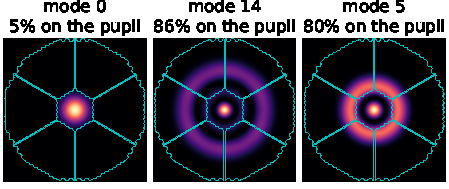
\includegraphics{pl19_800_modes_in_pupil}
\end{column}
\end{columns}
\end{frame}

\begin{frame}{\dots and what comes out of the 19 cores}
\centering
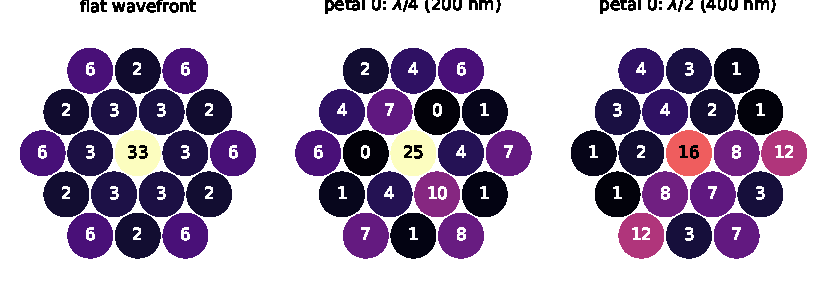
\includegraphics{pl19_800_output_face}
\begin{itemize}\small
    \item Same light, redistributed over the single-mode cores by the interference of the
          guided modes: the 19 numbers are the sensor signal.
    \item $\lambda/2$ of piston (right) is \emph{not} the flat case: at one wavelength a
          piston is seen modulo $\lambda$, and the response is periodic.
\end{itemize}
\end{frame}

% ===========================================================================
\section{Reconstructors at a single wavelength}
% ===========================================================================
\begin{frame}{The inverse problem}
\begin{itemize}
    \item Forward: pistons $\mathbf p \in \mathbb R^5$ $\to$ signals $\mathbf s = f(\mathbf p) \in \mathbb R^N$
          (smooth, nonlinear, periodic with period $\lambda$ in each piston).
    \item Reconstructor: $\hat{\mathbf p} = g(\mathbf s) \approx f^{-1}(\mathbf s)$, learned from
          simulated (or calibration) pairs $(\mathbf p, \mathbf s)$.
    \item At one wavelength the pistons must stay inside the \textbf{capture range}
          $\pm\lambda/2$; we use all of it: $\pm 400$~nm at 800~nm, $\pm 600$~nm at 1200~nm.
          At its edges $+\lambda/2$ and $-\lambda/2$ are the same piston: some cases are
          ambiguous for any reconstructor.
    \item Two known degeneracies:
    \begin{itemize}
        \item \textbf{periodicity}: $p$ and $p+\lambda$ give the same signals;
        \item \textbf{twin image}: $\varphi(x)$ and $-\varphi(-x)$ give the same focal
              \emph{intensity} -- broken by the lantern's mode mixing (not by a camera).
    \end{itemize}
    \item Evaluation: RMSE per piston on held-out samples (8000 train / 2000 validation,
          noiseless simulation unless stated).
\end{itemize}
\end{frame}

\begin{frame}{A family of reconstructors}
\small
\begin{tabular}{@{}p{0.23\linewidth}p{0.42\linewidth}p{0.28\linewidth}@{}}
\toprule
\textbf{Approach} & \textbf{Idea} & \textbf{Trade-off} \\
\midrule
Linear (interaction matrix) & push-pull calibration, $\hat{\mathbf p} = R(\mathbf s - \mathbf s_0)$ & simple, small range \\
Dense polynomial ridge & all monomials of degree $\le d$ & explainable; size $\sim N^d$ \\
Sparse polynomial (OMP) & keep the best $K$ monomials per piston & explainable, tunable size \\
Closed-form forward model & exact $|\!\sum\!|^2$ structure, Gauss-Newton inversion & physical; needs a good start \\
Symbolic regression & search for compact formulas (PySR) & readable; slow, approximate \\
Neural network (MLP) & learn $g$ directly & accurate; opaque, data hungry \\
\bottomrule
\end{tabular}
\vspace{4pt}
\begin{itemize}
    \item All trained on the same simulated datasets; ``degrees of freedom per piston''
          used as a common size measure.
\end{itemize}
\end{frame}

\begin{frame}{Linear reconstruction and calibration}
\begin{columns}[T]
\begin{column}{0.5\textwidth}
\small
\begin{itemize}
    \item Linearise: $\mathbf p \approx R\,(\mathbf s - \mathbf s_0)$; $R$ = (regularised)
          pseudo-inverse of the interaction matrix $B$.
    \item $B$ by push-pull on the DM:
          $B_{\cdot m} \approx [\mathbf s(+\delta) - \mathbf s(-\delta)]/2\delta$.
    \item Rank $\le N - 1$ (normalised signals).
    \item The reference $\mathbf s_0$ defines the convergence point.
    \item Linear range $\lesssim 1$ rad rms.
\end{itemize}
\end{column}
\begin{column}{0.5\textwidth}
\small
\begin{block}{19-port, 800 nm \oldrange}
Ridge-regularised linear reconstructor: \textbf{103 nm} rms\\
(no skill: 173 nm; $\pm300$ nm). The response over $\pm\lambda/2$ is far from linear $\Rightarrow$ nonlinear
reconstructors are needed.
\end{block}
\end{column}
\end{columns}
\end{frame}

\begin{frame}{Polynomial reconstructors: how many terms are needed?}
\begin{columns}[T]
\begin{column}{0.55\textwidth}
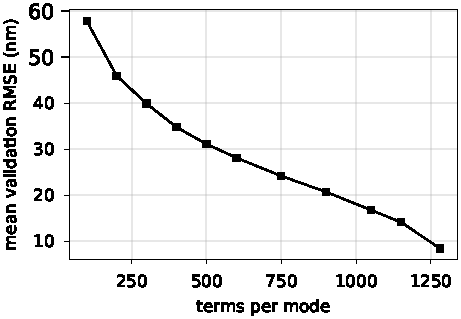
\includegraphics{pl19_800_omp_sweep}
\end{column}
\begin{column}{0.44\textwidth}
\small
\begin{itemize}
    \item Orthogonal Matching Pursuit keeps at most $K$ of the 1539 degree-$\le 3$ monomials
          of the 19 signals, per piston.
    \item The error falls smoothly with $K$ and \textbf{saturates at $K = 1281$}: every piston
          keeps its natural support; larger budgets reproduce the same fit (8.41~nm).
    \item $K = 1282$ (1281 terms + intercept) is the chosen budget.
    \item Dense quadratic: 56.5~nm; cubic is needed.
\end{itemize}
\end{column}
\end{columns}
\oldnote
\end{frame}

\begin{frame}{Neural network (MLP) reconstructor}
\begin{columns}[T]
\begin{column}{0.58\textwidth}
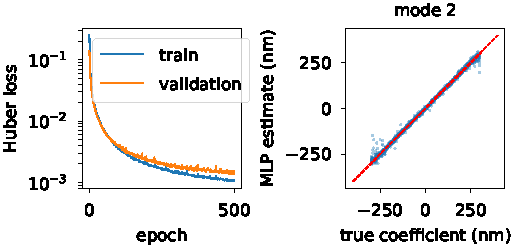
\includegraphics{pl19_800_mlp_training}
\end{column}
\begin{column}{0.41\textwidth}
\small
\begin{itemize}
    \item $19 \to 3\times128 \to 5$, Adam, 500 epochs, best validation epoch kept:
          \textbf{9.0 nm}.
    \item Hyperparameter search (4$\times$256, cosine schedule): $\sim$4.3 nm on the same data;
          more data helps more than bigger networks (appendix).
    \item Errors are heavy-tailed: median $\ll$ RMSE.
\end{itemize}
\end{column}
\end{columns}
\oldnote
\end{frame}

\begin{frame}{Single wavelength: comparison (19 ports, 800 nm, $\pm\lambda/2$)}
\begin{columns}[T]
\begin{column}{0.62\textwidth}
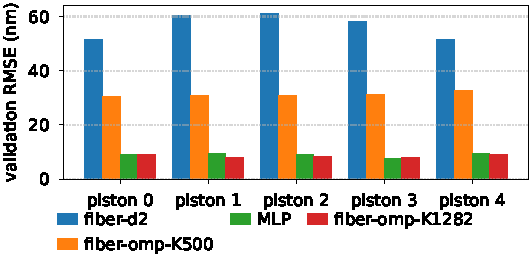
\includegraphics{pl19_800_single_comparison}
\end{column}
\begin{column}{0.37\textwidth}
\small
\begin{tabular}{@{}lr@{}}
\toprule
reconstructor & RMSE (nm) \\
\midrule
no skill & 173 \\
linear & 103.1 \\
dense quadratic & 56.5 \\
OMP cubic, $K{=}500$ & 31.1 \\
\textbf{MLP} & \textbf{9.0} \\
\textbf{OMP cubic, $K{=}1282$} & \textbf{8.4} \\
\bottomrule
\end{tabular}
\vspace{4pt}

A sparse cubic polynomial matches the MLP with $\sim$6$\times$ fewer parameters.
\end{column}
\end{columns}
\oldnote
\end{frame}

\begin{frame}{Physics-based and symbolic reconstructors}
\begin{columns}[T]
\begin{column}{0.5\textwidth}
\small
\begin{itemize}
    \item \textbf{Closed form}: with petal pistons the signals are exactly quadratic forms in
          the petal phasors, $s_k = \sum_{j,j'} e^{i(\theta_j-\theta_{j'})} H^{(k)}_{jj'}$:
          619 constants for 19 cores and 6 petals, fitted from data.
    \item Inverted by Gauss-Newton from a few starts; converges to $\ll$ 1 nm noiseless.
    \item \textbf{Symbolic regression} (PySR, Operon) finds compact per-piston formulas;
          useful for insight, less accurate.
\end{itemize}
\placeholder{decide how much of the closed-form / symbolic work goes in the main talk vs appendix; add its accuracy-vs-noise numbers.}
\end{column}
\begin{column}{0.5\textwidth}
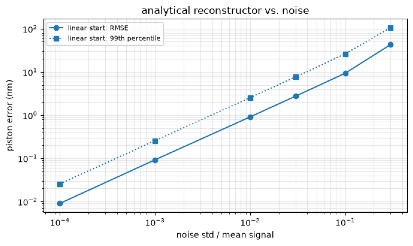
\includegraphics{pl19_800_forward_model_noise}\\
{\scriptsize closed-form model: error vs. signal noise (19 ports, 800 nm)}
\end{column}
\end{columns}
\oldnote
\end{frame}

% ===========================================================================
\section{Case study: ANDES petal pistons with a dispersed lantern}
% ===========================================================================
\begin{frame}{ANDES and the petal problem}
\begin{columns}[T]
\begin{column}{0.55\textwidth}
\small
\begin{itemize}
    \item ELT pupil: the spiders split it into \textbf{6 petals}; differential pistons between
          them (``petal modes'') are poorly sensed by the pyramid WFS and can be large
          (low-wind effect, M4 segment phasing).
    \item We consider 5 petal pistons (the 6th petal as reference), from the ANDES DM modal
          basis.
    \item Target: sense pistons over \textbf{many waves} ($\pm 8\lambda$: $\pm6.4\,\mu$m at
          800 nm, $\pm9.6\,\mu$m at 1200 nm), not only inside $\pm\lambda/2$.
\end{itemize}
\placeholder{ANDES-specific requirements: expected petal piston amplitudes and temporal behaviour, wavelength band available for sensing, required accuracy (nm) and photon budget -- from the ANDES AO/SCAO team.}
\end{column}
\begin{column}{0.44\textwidth}
\centering
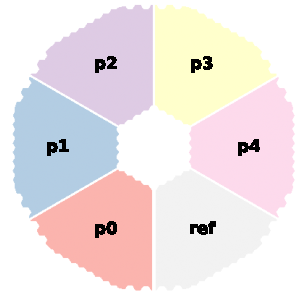
\includegraphics{pl19_800_pupil_petals}
\end{column}
\end{columns}
\end{frame}

\begin{frame}{Beyond $\pm\lambda/2$: the dispersed lantern}
\begin{columns}[T]
\begin{column}{0.5\textwidth}
\small
\begin{itemize}
    \item At one wavelength a piston is known only modulo $\lambda$.
    \item Feed the $N$ lantern outputs to a spectrograph slit: each core gives a
          \textbf{spectrum}, i.e.\ the signals at many wavelengths at once.
    \item Different $\lambda$ wrap differently $\Rightarrow$ synthetic-wavelength
          interferometry can resolve the full range.
    \item We simulate 41 wavelengths (5 nm steps) over the band; the power of each core
          at each wavelength, as a fraction of the incident power.
\end{itemize}
\end{column}
\begin{column}{0.5\textwidth}
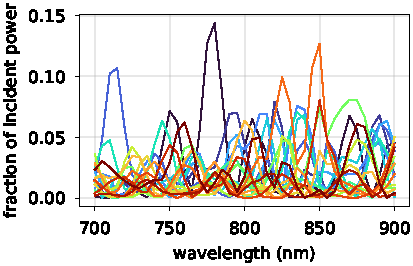
\includegraphics{pl19_800_sample_spectra}\\
{\scriptsize one random $\pm8\lambda$ configuration: the 19 core spectra (19 ports, 700--900 nm)}
\end{column}
\end{columns}
\end{frame}

\begin{frame}{Spectral response to one petal piston}
\begin{columns}[T]
\begin{column}{0.55\textwidth}
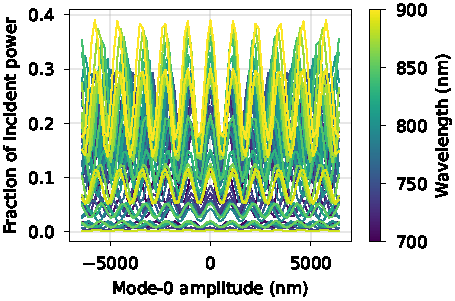
\includegraphics{pl19_800_core0_ramp}
\end{column}
\begin{column}{0.44\textwidth}
\small
\begin{itemize}
    \item Petal 0 ramped over $\pm 8\lambda$ ($\pm6.4\,\mu$m); the central core's signal at
          each of the 41 wavelengths.
    \item Each wavelength is periodic in the piston with its own period $\lambda$: the
          combination is unique over the range.
\end{itemize}
{\scriptsize The same response for the 1200 nm lanterns: appendix.}
\end{column}
\end{columns}
\end{frame}

\begin{frame}{Three lanterns}
\small
\centering
\resizebox{\linewidth}{!}{%
\begin{tabular}{@{}lccc@{}}
\toprule
 & \textbf{pl19\_800} (reference) & \textbf{pl7\_1200} & \textbf{pl19\_1200} \\
\midrule
ports & 19 & 7 (1 + 6 hexagon) & 19 \\
design $\lambda$ / band & 800 / 700--900 nm & 1200 / 1100--1300 nm & 1200 / 1100--1300 nm \\
cladding / core / jacket $\Delta n$ & 1.444 / $+8.8$ / $-5.5\,(10^{-3})$ & 1.4481 / $+5.0$ / $-10\,(10^{-3})$ & as pl7\_1200 \\
multimode NA, radius & 0.126, 9.0 $\mu$m & 0.170, 6.4 $\mu$m & 0.170, 10.0 $\mu$m \\
$V$ at design $\lambda$ & 8.90 & 5.69 & 8.90 \\
guided modes (blue / centre / red) & 30 / 23 / 17 & 10 / 10 / 8 & 23 / 23 / 17 \\
taper, length & $\times12$, 100 mm & $\times15$, 100 mm & $\times15$, 100 mm \\
flat-wavefront coupling & 34--53\% & 41--57\% & 36--50\% \\
\bottomrule
\end{tabular}}
\vspace{6pt}
\begin{itemize}
    \item The 1200 nm lanterns share one fibre technology (Ge-doped SMF-like cores,
          F-doped capillary); \textbf{only the port count differs} between them.
    \item Same PSF sizing rule for all: beam NA / multimode NA as in the reference.
\end{itemize}
\end{frame}

\begin{frame}{Design choices at 1200 nm}
\begin{columns}[T]
\begin{column}{0.52\textwidth}
\small
\begin{itemize}
    \item Multimode end sized to the port count: $\sim N$ (to $N{+}4$) guided modes.
    \item 7 ports: LP$_{31}$ comes as a pair; $V$ chosen so it stays guided to 1300 nm.
    \item Output cores: 6.6 $\mu$m, single-mode over the band; pitch 60 $\mu$m (uncoupled).
    \item Mode bookkeeping (degenerate pairs, dropped mode) checked by FEM every 25 nm.
    \item Mesh: $\Delta n_\mathrm{eff} \le 1.6\times10^{-5}$ when doubled.
\end{itemize}
\end{column}
\begin{column}{0.46\textwidth}
\small
\begin{block}{7-port cladding radius (FEM)}
\begin{tabular}{@{}lccc@{}}
$r_\mathrm{clad}$ & 1100 & 1200 & 1300 nm \\
\midrule
6.2 $\mu$m & 10 & 10 & \textcolor{red}{6} \\
\textbf{6.4 $\mu$m} & 10 & 10 & \textbf{8} \\
6.6 $\mu$m & 12 & 10 & 8 \\
\end{tabular}
\vspace{2pt}

guided modes at the multimode end
\end{block}
\placeholder{design references: Lin et al.\ 2022/2023 (6- and 19-port lanterns, $V\approx5.1$ and 9.6); Birks et al.\ 2015.}
\end{column}
\end{columns}
\end{frame}

\begin{frame}{Simulation campaign}
\begin{itemize}
    \item Per lantern: 41 characterizations (one per wavelength) $\to$ two datasets:
    \begin{itemize}
        \item \textbf{single wavelength}: 10\,000 random 5-piston configurations, camera signals
              of the cores at the design $\lambda$, $\pm\lambda/2$ ($\pm400$ nm at 800 nm, $\pm600$ nm at 1200 nm);
        \item \textbf{spectral}: 50\,000 configurations, $\pm 8\lambda$ ($\pm6.4$ / $\pm9.6\,\mu$m),
              core powers at 41 wavelengths ($\lambda \pm 100$ nm).
    \end{itemize}
    \item 40\,000 / 10\,000 train / validation; all reconstructors trained on identical data.
    \item Runs on CINECA Leonardo (Booster): the 41 characterizations and the dataset pieces
          spread over whole nodes, $\le 8$ nodes at a time; first campaign on a 64-core / 2-GPU server.
    \item One code base, lantern chosen by a preset name; executed notebooks kept per lantern.
\end{itemize}
\placeholder{add photon noise / detector noise and a spectrograph model (the \texttt{spectral} package exists; not yet in the reconstruction study).}
\end{frame}

% ===========================================================================
\section{Piston sensing with a dispersed lantern: comparison of approaches}
% ===========================================================================
\begin{frame}{Two strategies for many wavelengths}
\begin{columns}[T]
\begin{column}{0.5\textwidth}
\begin{block}{A. One model on the whole spectrum}
\small
Input: all $41\times N$ signals; output: the 5 pistons directly.\\
Linear, dense quadratic ridge (wavelength subset), global sparse cubic (OMP), MLP.
\end{block}
\end{column}
\begin{column}{0.5\textwidth}
\begin{block}{B. Per wavelength, then unwrap}
\small
At each $\lambda$: a small model regresses each piston's \emph{phasor}
$(\sin,\cos)(2\pi p/\lambda)$ -- smooth, bounded, one fringe.\\
Then a multi-wavelength unwrap (circular maximum likelihood over $\pm8\lambda$ + robust
refinement) fuses the wrapped estimates, as in synthetic-wavelength interferometry.
\end{block}
\end{column}
\end{columns}
\vspace{6pt}
\begin{itemize}
    \item B with sparse cubic polynomials (OMP) or small MLPs per wavelength.
    \item A ``wrong fringe'': error larger than half the shortest wavelength.
\end{itemize}
\end{frame}

\begin{frame}{Per-wavelength models (19 ports, 700--900 nm)}
\centering
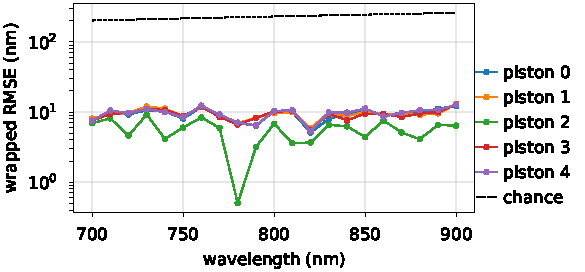
\includegraphics{pl19_800_wrapped_rmse}\\
{\scriptsize wrapped-piston RMSE of each per-wavelength model (dashed: chance)}
\begin{itemize}\small
    \item Each per-wavelength model gets the wrapped piston (one fringe) to a few nm.
\end{itemize}
\oldnote
\end{frame}

\begin{frame}{The multi-wavelength unwrap (19 ports, 700--900 nm)}
\centering
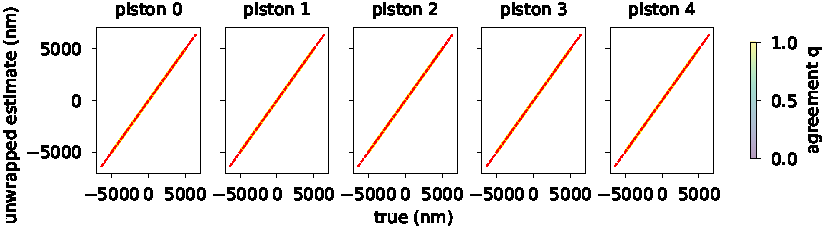
\includegraphics{pl19_800_unwrap_scatter}\\
{\scriptsize unwrapped estimate vs.\ truth over the full $\pm8\lambda$, one panel per piston}
\begin{itemize}\small
    \item The unwrap fuses the wrapped estimates of the 41 wavelengths and recovers the full
          range with \textbf{no wrong fringes}: \textbf{1.64 nm} rms.
\end{itemize}
\oldnote
\end{frame}

\begin{frame}{Comparison, reference lantern (19 ports, 700--900 nm, $\pm 8\lambda$)}
\begin{columns}[T]
\begin{column}{0.6\textwidth}
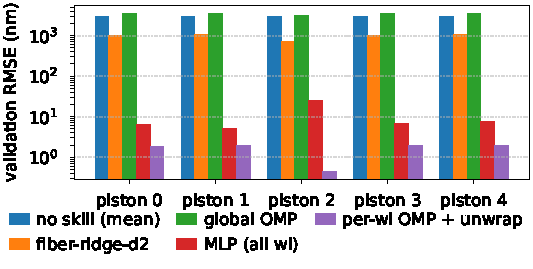
\includegraphics{pl19_800_spectral_comparison}
\end{column}
\begin{column}{0.39\textwidth}
\small
\begin{tabular}{@{}lr@{}}
\toprule
approach & RMSE (nm) \\
\midrule
no skill & 2893 \\
global OMP (3 $\lambda$) & 3420 \\
linear & 2809 \\
dense quadratic & 969 \\
MLP, full spectrum & 10.25 \\
\textbf{per-$\lambda$ OMP + unwrap} & \textbf{1.64} \\
per-$\lambda$ MLP + unwrap & 0.44--1.0 \\
\bottomrule
\end{tabular}
\vspace{3pt}

{\scriptsize last row: hyperparameter search, held-out protocol}
\end{column}
\end{columns}
\oldnote
\end{frame}

\begin{frame}{7 ports at 1200 nm: results}
\begin{columns}[T]
\begin{column}{0.5\textwidth}
\small
\begin{tabular}{@{}lrr@{}}
\toprule
 & single $\lambda$ & spectral \\
 & $\pm\lambda/2$ & $\pm8\lambda$ \\
\midrule
no skill & 288 & 2893 \\
linear & 261.9 & 2852 \\
dense quadratic & 243.2 & 1488 \\
OMP (cubic / global) & 228.5 & 2249 \\
MLP & 226.4 & \textbf{278.0} \\
per-$\lambda$ OMP + unwrap & -- & 1665 \\
\bottomrule
\end{tabular}
\vspace{4pt}

{\scriptsize nm rms, validation set. $r_\mathrm{clad}$ = 6.4 $\mu$m; the earlier 6.2 $\mu$m design
gave 221.8 / 257.8 / 1688 nm for the MLP / full-spectrum MLP / unwrap: the redesign changes little.}
\end{column}
\begin{column}{0.5\textwidth}
\small
\begin{itemize}
    \item One wavelength: every reconstructor stops at $\sim$230 nm (no skill 288); the cubic
          OMP sweep is flat (260 $\to$ 229 nm from $K$ = 5 to 119): the model is not the limit.
    \item Spectral: the per-wavelength route \textbf{fails} -- 53\% of the estimates on a wrong
          fringe; only the full-spectrum MLP learns (10$\times$ better than no skill; still
          improving at its last epoch).
    \item Flat-wavefront coupling 41--57\% over the band.
\end{itemize}
\end{column}
\end{columns}
\oldnote
\end{frame}

\begin{frame}{7 ports at 1200 nm: per piston}
\begin{columns}[T]
\begin{column}{0.5\textwidth}
\centering
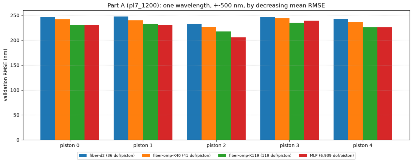
\includegraphics{pl7_1200_single_comparison}\\
{\scriptsize one wavelength (1200 nm), $\pm\lambda/2$}
\end{column}
\begin{column}{0.5\textwidth}
\centering
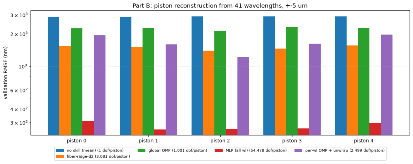
\includegraphics{pl7_1200_spectral_comparison}\\
{\scriptsize 41 wavelengths (1100--1300 nm), $\pm8\lambda$ (log scale)}
\end{column}
\end{columns}
{\scriptsize Per-wavelength models and their unwrap: appendix.}
\oldnote
\end{frame}

\begin{frame}{19 ports at 1200 nm: results}
\begin{columns}[T]
\begin{column}{0.5\textwidth}
\small
\begin{tabular}{@{}lrr@{}}
\toprule
 & single $\lambda$ & spectral \\
 & $\pm\lambda/2$ & $\pm8\lambda$ \\
\midrule
no skill & 288 & 2893 \\
linear & 213.3 & 2767 \\
dense quadratic & 117.1 & 397 \\
OMP (cubic $K{=}1282$ / global) & 31.9 & 1827 \\
MLP & \textbf{25.9} & \textbf{9.48} \\
per-$\lambda$ OMP + unwrap & -- & 30.0 \\
\bottomrule
\end{tabular}
\vspace{4pt}

{\scriptsize nm rms, validation set; same fibres, wavelength and data as pl7\_1200 -- only the port count differs.}
\end{column}
\begin{column}{0.5\textwidth}
\small
\begin{itemize}
    \item 19 ports restore the performance: \textbf{9.5 nm} over the spectral range with the
          full-spectrum MLP (7 ports: 278 nm; reference lantern: 10.25 nm).
    \item One wavelength: 26--32 nm. In the first campaign not directly comparable with the
          reference's 8--9 nm ($\pm0.375\lambda$ vs $\pm0.42\lambda$); the rerun uses $\pm\lambda/2$ for both.
    \item Per-$\lambda$ OMP + unwrap: the bulk of the estimates is at the nm level (piston 2:
          0.65 nm), but $\sim$1 in 1000 lands on a wrong fringe and dominates the RMSE (30 nm).
\end{itemize}
\end{column}
\end{columns}
\oldnote
\end{frame}

\begin{frame}{19 ports at 1200 nm: per piston}
\begin{columns}[T]
\begin{column}{0.5\textwidth}
\centering
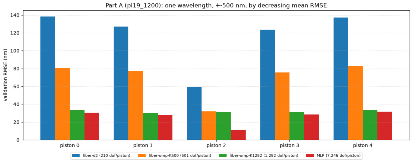
\includegraphics{pl19_1200_single_comparison}\\
{\scriptsize one wavelength (1200 nm), $\pm\lambda/2$}
\end{column}
\begin{column}{0.5\textwidth}
\centering
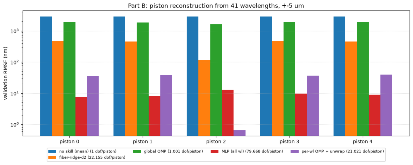
\includegraphics{pl19_1200_spectral_comparison}\\
{\scriptsize 41 wavelengths (1100--1300 nm), $\pm8\lambda$ (log scale)}
\end{column}
\end{columns}
{\scriptsize Per-wavelength models and their unwrap: appendix.}
\oldnote
\end{frame}

\begin{frame}{Why do 7 ports fail? Not resolution: uniqueness}
\begin{columns}[T]
\begin{column}{0.53\textwidth}
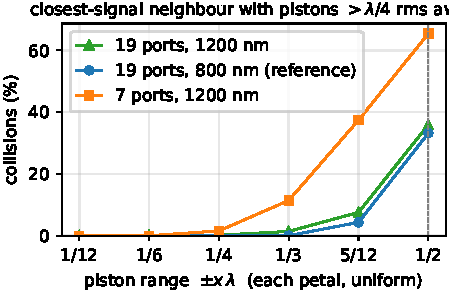
\includegraphics{ambiguity_vs_range}
\end{column}
\begin{column}{0.46\textwidth}
\small
\begin{itemize}
    \item Test, no reconstructor involved: 3000 random piston sets per range; for each, the
          set with the closest signals. A \textbf{collision} = their pistons differ by
          $>\lambda/4$ rms (the signals point to a wrong solution).
    \item Locally the 7-port is fine (full-rank Jacobian, twin image broken); no collisions
          up to $\pm\lambda/6$.
    \item Up to $\pm5\lambda/12$: \textbf{37\%} collisions with 7 ports, 7.6\% with 19 ports in
          the same fibres, 4.3\% for the reference.
    \item At the study's $\pm\lambda/2$ (dashed) the wrap adds its own: $+\lambda/2 \equiv -\lambda/2$.
          \textbf{65\%} with 7 ports, 36\% / 33\% with 19 ports.
    \item About 1/3 of the collisions are twin-image pairs; the rest are other folds.
\end{itemize}
\end{column}
\end{columns}
\end{frame}

\begin{frame}{Why do 7 ports fail? Counting dimensions}
\begin{itemize}
    \item The 5 pistons live on a 5-dimensional torus (each wraps with $\lambda$).
    \item An $N$-port lantern gives $N-1$ independent normalised signals per wavelength.
    \item A smooth map of a 5-dimensional space is in general one-to-one only into
          $\ge 2\cdot 5 + 1 = 11$ dimensions (Whitney); into fewer it folds onto itself,
          with families of colliding configurations of dimension $2\cdot5 - (N-1)$.
    \item \textbf{19 ports: 18 $\ge$ 11} $\Rightarrow$ unique. \textbf{7 ports: 6 $<$ 11}
          $\Rightarrow$ 4-dimensional families of piston sets with identical signals.
    \item Consistent with the literature: an $N$-port lantern senses at most $\sim N-1$ modes
          per frame (Lin et al.\ 2022, 2023).
    \item Per-wavelength models see the pistons wrapped over a full $\pm\lambda/2$ $\Rightarrow$
          they inherit the ambiguity; a model of the whole spectrum ($41\times6$ numbers)
          can still partly resolve it.
\end{itemize}
\begin{block}{Confirmed by the 1200 nm pair}
\small Same fibres, same wavelength, only the port count differs: at $\pm5\lambda/12$ the collisions drop
from 37\% (7 ports) to 7.6\% (19 ports), at $\pm\lambda/2$ from 65\% to 36\%; the best spectral
reconstruction from 278 nm to 9.5 nm \oldrange.
\end{block}
\end{frame}

\begin{frame}{Model size vs accuracy (19 ports, MLP hyperparameter search)}
\begin{columns}[T]
\begin{column}{0.62\textwidth}
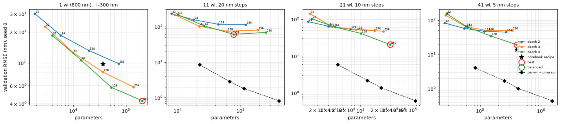
\includegraphics{pl19_800_hpo_grid}
\end{column}
\begin{column}{0.37\textwidth}
\small
\begin{itemize}
    \item Full-spectrum MLPs need depth and are hard to train (seed spread).
    \item Per-wavelength MLPs + unwrap: 0.44--1.0 nm, also with 20 nm steps (11 wavelengths).
\end{itemize}
\placeholder{repeat the search for pl7\_1200 / pl19\_1200 (needs porting \texttt{scripts/mlp\_hpo.py}).}
\end{column}
\end{columns}
\oldnote
\end{frame}

\begin{frame}{Comparison across lanterns}
\small
\centering
\begin{tabular}{@{}lccc@{}}
\toprule
RMSE (nm) & pl19\_800 & pl7\_1200 & pl19\_1200 \\
\midrule
single $\lambda$, best (MLP / OMP) & 9.0 / 8.4 & 226.4 / 228.5 & 25.9 / 31.9 \\
single $\lambda$, no skill & 173 & 288 & 288 \\
single $\lambda$, range (rerun) & $\pm\lambda/2$ & $\pm\lambda/2$ & $\pm\lambda/2$ \\
collisions at $\pm\lambda/2$ & 33\% & 65\% & 36\% \\
collisions at $\pm5\lambda/12$ & 4.3\% & 37\% & 7.6\% \\
spectral, full-spectrum MLP & 10.25 & 278.0 & \textbf{9.48} \\
spectral, per-$\lambda$ OMP + unwrap & 1.64 & 1665 (53\% wrong) & 30.0 (0.08\% wrong) \\
spectral, no skill & 2893 & 2893 & 2893 \\
\bottomrule
\end{tabular}
\vspace{8pt}
\placeholder{robustness: photon noise, read noise, calibration errors, wavelength sampling (20/10/5 nm), lantern manufacturing variations.}
\oldnote
\end{frame}

% ===========================================================================
\section{Conclusions}
% ===========================================================================
\begin{frame}{Conclusions (so far)}
\begin{enumerate}
    \item A photonic lantern turns the focal-plane field into $N$ intensities through fixed
          modal interference; simulated end-to-end with coupled-mode theory (cbeam).
    \item At one wavelength, a 19-port lantern supports nonlinear reconstructors at
          $\sim$8--9 nm over $\pm0.375\lambda$ \oldrange; sparse cubic polynomials match MLPs.
          Over the full $\pm\lambda/2$ the wrap at the edges adds unavoidable ambiguous cases.
    \item Dispersing the outputs extends the range to many waves: per-wavelength models +
          unwrap reach $\sim$1--2 nm over $\pm 5\,\mu$m (19 ports) \oldrange.
    \item The \textbf{port count} matters: with 7 ports the signals are not unique over a
          large range; only joint use of all wavelengths partly helps (278 nm \oldrange).
    \item At 1200 nm with the same fibres, 19 ports bring the spectral error back to $\sim$10 nm
          (7 ports: 278 nm) \oldrange: the port count, not the wavelength or the fibres,
          sets the limit.
    \item \placeholder{recommendation for ANDES (with the team).}
\end{enumerate}
\end{frame}

\begin{frame}{Next steps}
\begin{itemize}
    \item MLP hyperparameter search for pl7\_1200 and pl19\_1200 (port \texttt{scripts/mlp\_hpo.py}).
    \item Noise: photon / read noise through the spectrograph model; required flux.
    \item Calibration on a real device: how many calibration samples does each approach need?
    \item Sensitivity to fabrication: random lanterns of the same design.
    \item Closed loop with the ANDES AO simulation.
    \item \placeholder{others from the team.}
\end{itemize}
\end{frame}

\appendix
% ===========================================================================
\section*{Appendix}
% ===========================================================================
\begin{frame}{Appendix: more on the lantern response}
\begin{columns}[T]
\begin{column}{0.48\textwidth}
\centering
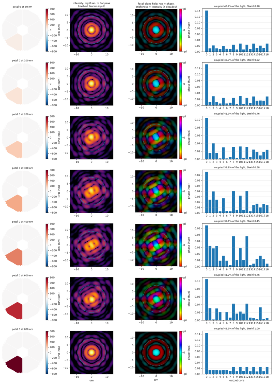
\includegraphics{pl19_800_psf_zoo_piston}
\end{column}
\begin{column}{0.5\textwidth}
\small
\begin{itemize}
    \item Petal 0 from 50 to 800 nm: pupil, focal-plane intensity and phase, power in each
          output core (19 ports, 800 nm).
    \item At 800 nm (one wave) the response returns to the flat one.
\end{itemize}
\oldnote
\end{column}
\end{columns}
\end{frame}

\begin{frame}{Appendix: twin pairs}
\centering
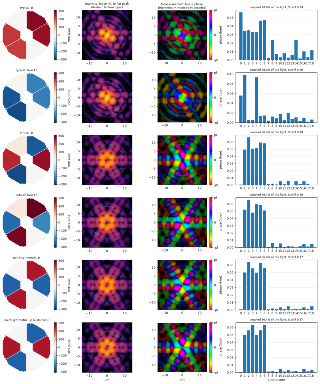
\includegraphics{pl19_800_psf_zoo_twins}
\end{frame}

\begin{frame}{Appendix: PSF size and coupling}
\begin{itemize}
    \item The PSF is sized so that the Airy first-null radius is $0.30\,r_\mathrm{clad}$ for the
          reference lantern; the 1200 nm lanterns keep the same beam-NA / fibre-NA ratio
          (fill $= 0.30\,V_\mathrm{ref}/V$).
    \item This overfills the fibre NA by $\sim$1.4$\times$: flat-wavefront coupling $\sim$45\%,
          vs.\ $\sim$90\% for a throughput-optimised focal ratio (Lin et al.\ 2023).
    \item Kept for comparability with the reference; its effect on sensing is to be studied.
\end{itemize}
\placeholder{scan of reconstruction accuracy and coupling vs.\ focal ratio.}
\end{frame}

\begin{frame}{Appendix: OMP -- which monomials are kept?}
\centering
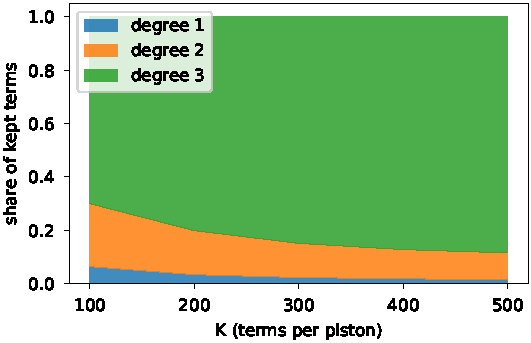
\includegraphics{pl19_800_omp_degree_mix}
\end{frame}

\begin{frame}{Appendix: more data vs bigger networks (19 ports, 800 nm)}
\centering
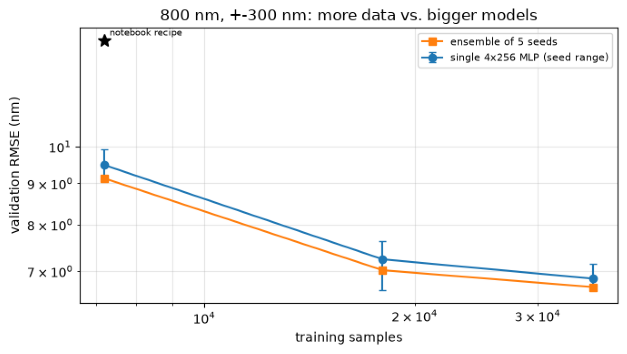
\includegraphics{pl19_800_more_data}
\end{frame}

\begin{frame}{Appendix: linear sensitivity of each wavelength to each piston}
\centering
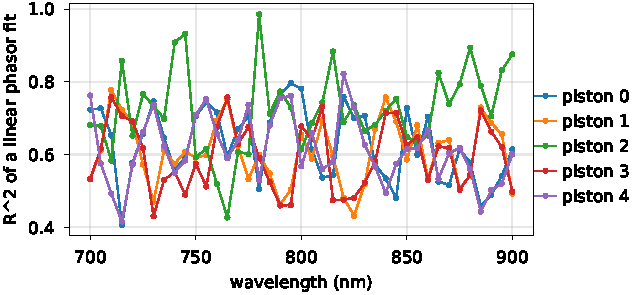
\includegraphics{pl19_800_phasor_r2}
\end{frame}

\begin{frame}{Appendix: 7 ports at 1200 nm in simulation}
\begin{columns}[T]
\begin{column}{0.5\textwidth}
\centering
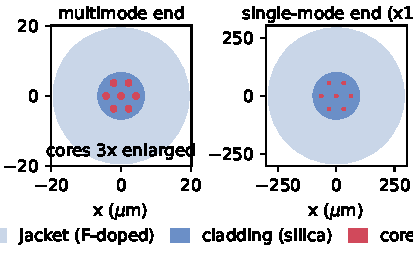
\includegraphics{pl7_1200_geometry}
\end{column}
\begin{column}{0.5\textwidth}
\centering
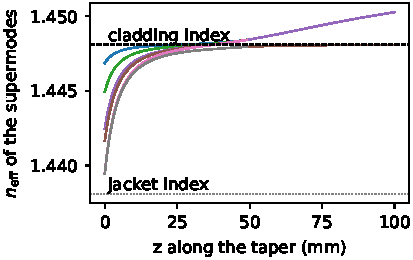
\includegraphics{pl7_1200_neff_vs_z}
\end{column}
\end{columns}
\end{frame}

\begin{frame}{Appendix: one petal piston through the 7-port lantern at 1200 nm}
\centering
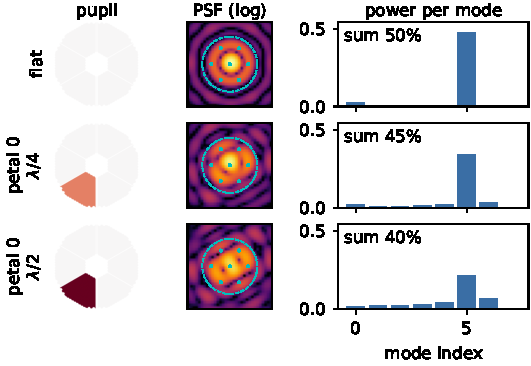
\includegraphics{pl7_1200_psf_coupling}
\end{frame}

\begin{frame}{Appendix: 7-port lantern at 1200 nm, output face}
\centering
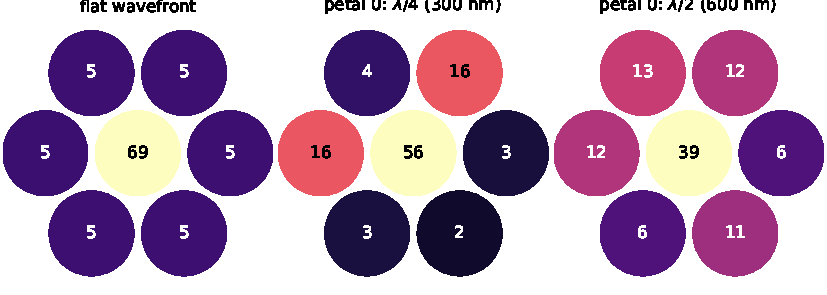
\includegraphics{pl7_1200_output_face}
\end{frame}

\begin{frame}{Appendix: 19 ports at 1200 nm in simulation}
\begin{columns}[T]
\begin{column}{0.5\textwidth}
\centering
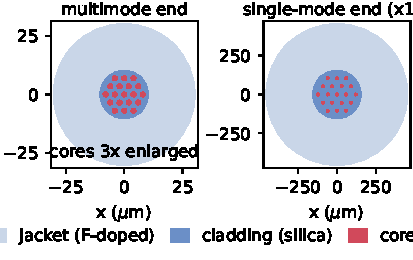
\includegraphics{pl19_1200_geometry}
\end{column}
\begin{column}{0.5\textwidth}
\centering
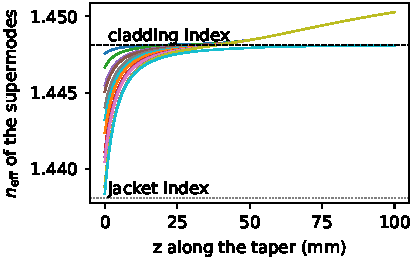
\includegraphics{pl19_1200_neff_vs_z}
\end{column}
\end{columns}
\end{frame}

\begin{frame}{Appendix: one petal piston through the 19-port lantern at 1200 nm}
\centering
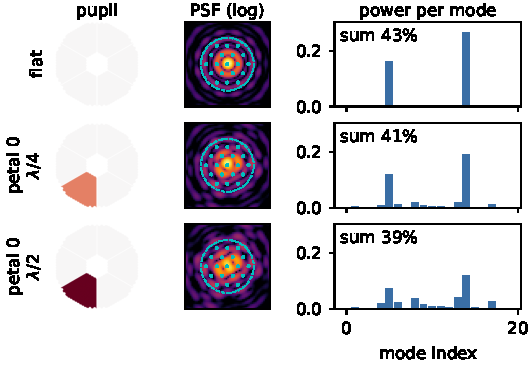
\includegraphics{pl19_1200_psf_coupling}
\end{frame}

\begin{frame}{Appendix: 19-port lantern at 1200 nm, output face}
\centering
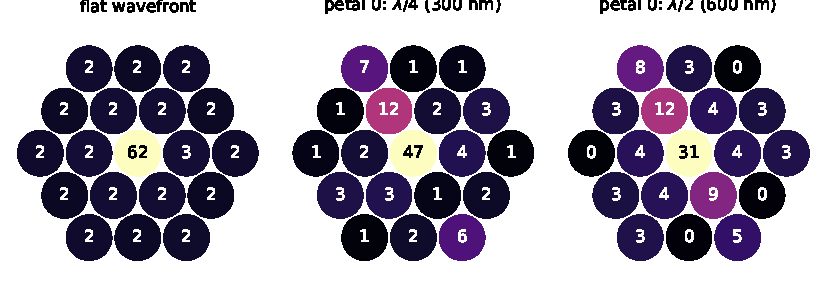
\includegraphics{pl19_1200_output_face}
\end{frame}

\begin{frame}{Appendix: 19 ports at 1200 nm, per-wavelength models}
\centering
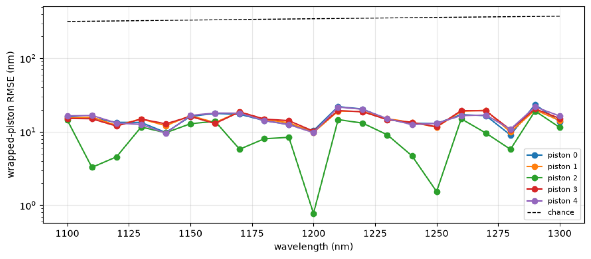
\includegraphics{pl19_1200_wrapped_rmse}\\
{\scriptsize per-wavelength models: wrapped-piston error (dashed: chance)}
\oldnote
\end{frame}

\begin{frame}{Appendix: 19 ports at 1200 nm, the unwrap}
\centering
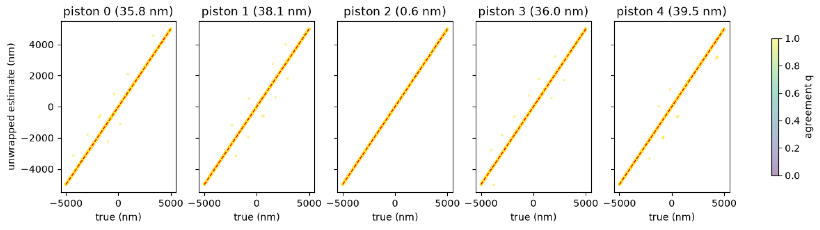
\includegraphics{pl19_1200_unwrap_scatter}\\
{\scriptsize unwrap: a few wrong-fringe outliers per piston}
\oldnote
\end{frame}

\begin{frame}{Appendix: 19 ports at 1200 nm, spectral response}
\begin{columns}[T]
\begin{column}{0.5\textwidth}
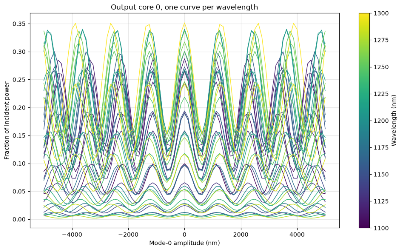
\includegraphics{pl19_1200_core0_ramp}\\
{\scriptsize central core, one petal ramped over $\pm8\lambda$ ($\pm9.6\,\mu$m), one curve per wavelength}
\end{column}
\begin{column}{0.5\textwidth}
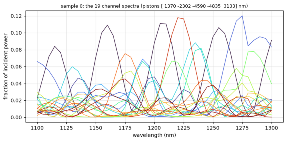
\includegraphics{pl19_1200_sample_spectra}\\
{\scriptsize one random configuration: the 19 core spectra}\\[6pt]
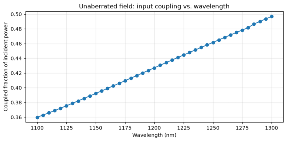
\includegraphics{pl19_1200_coupling_vs_wl}\\
{\scriptsize flat-wavefront coupling vs.\ wavelength}
\end{column}
\end{columns}
\end{frame}

\begin{frame}{Appendix: 7 ports at 1200 nm, per-wavelength models}
\centering
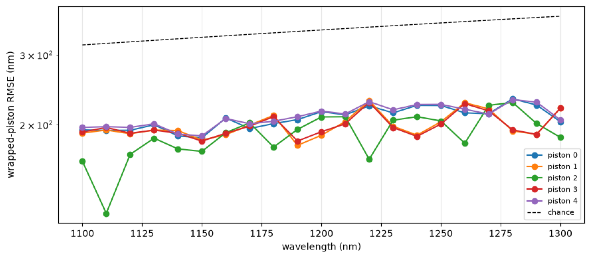
\includegraphics{pl7_1200_wrapped_rmse}\\
{\scriptsize per-wavelength models: wrapped-piston error $\sim$200 nm (dashed: chance)}
\oldnote
\end{frame}

\begin{frame}{Appendix: 7 ports at 1200 nm, the unwrap}
\centering
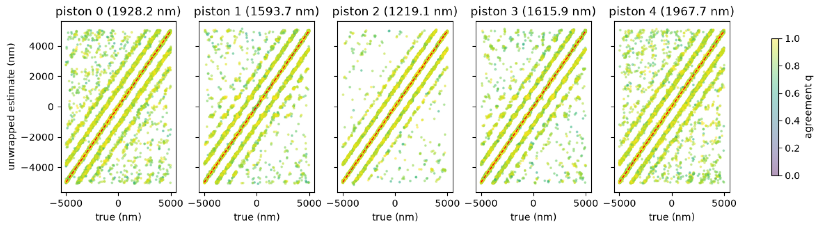
\includegraphics{pl7_1200_unwrap_scatter}\\
{\scriptsize the unwrap then lands on wrong fringes}
\oldnote
\end{frame}

\begin{frame}{Appendix: 7 ports at 1200 nm, spectral response}
\begin{columns}[T]
\begin{column}{0.5\textwidth}
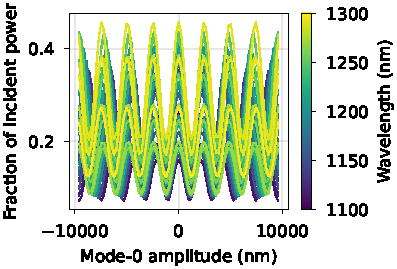
\includegraphics{pl7_1200_core0_ramp}\\
{\scriptsize central core, one petal ramped over $\pm8\lambda$ ($\pm9.6\,\mu$m), one curve per wavelength}
\end{column}
\begin{column}{0.5\textwidth}
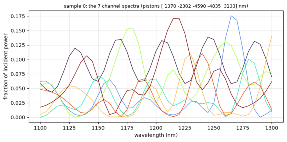
\includegraphics{pl7_1200_sample_spectra}\\
{\scriptsize one random configuration: the 7 core spectra}\\[6pt]
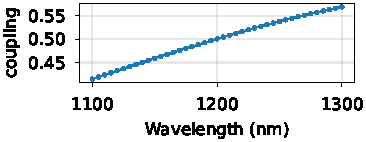
\includegraphics{pl7_1200_coupling_vs_wl}\\
{\scriptsize flat-wavefront coupling vs.\ wavelength}
\end{column}
\end{columns}
\end{frame}

% --- the tutorial material of the original deck, kept for reference ---------
\begin{frame}{Appendix: from Maxwell to the paraxial equation}
\begin{itemize}
    \item Scalar Helmholtz equation (weakly guiding): $\nabla^2 E + k_0^2 n^2 E = 0$.
    \item Paraxial wave equation for the envelope $u$:
    \[ \frac{\partial u}{\partial z} = \frac{i}{2 k_0 n_0}\left[\nabla_\perp^2 + k_0^2 (n^2 - n_0^2)\right] u \]
    \item Pupil to focus: $E = \mathcal F[P e^{i\varphi}]$, unitary; aberrations on Zernikes,
          even or odd under inversion.
\end{itemize}
\end{frame}

\begin{frame}{Appendix: coupled-mode theory and adiabaticity}
\begin{itemize}
    \item $\dfrac{d a_m}{dz} = i\beta_m a_m - \sum_n \kappa_{mn} a_n$, \quad
          $\kappa_{mn} = \langle \xi_m | \partial_z \xi_n \rangle$ (antisymmetric).
    \item Adiabatic if $|\kappa_{mn}| \ll |\beta_n - \beta_m|$ everywhere; Hellmann-Feynman:
          $\kappa_{mn} = k_0^2 \langle \xi_m|\partial_z\varepsilon|\xi_n\rangle/(\beta_n^2-\beta_m^2)$.
    \item Degenerate pairs aligned by an orthogonal Procrustes step; near the single-mode end
          the levels merge and the evolution freezes.
    \item CMT keeps only guided modes (no radiation loss); validate against BPM per design family.
\end{itemize}
\end{frame}

\begin{frame}{Appendix: wavelength scaling and the sensor as one matrix}
\begin{itemize}
    \item Similarity: $A(\lambda, G) = A(\sigma\lambda, \sigma G)$ if \emph{all} lengths scale,
          including the taper length; material dispersion breaks it.
    \item Back-propagate the guided modes to the pupil: $\mathbf p = |A M \mathbf f|^2 = |C\mathbf f|^2$,
          one precomputed matrix $C(\lambda)$ per wavelength -- cheap inside an AO simulation.
    \item Light outside the $N$ modes ($1 - \sum|u_n|^2$) is lost to both sensor and science fibres.
\end{itemize}
\end{frame}

\begin{frame}{Appendix: experimental record}
\small
\centering
\begin{tabular}{@{}lll@{}}
\toprule
\textbf{Year} & \textbf{Reference} & \textbf{Result} \\
\midrule
2025 & Lin et al. & On-sky spectral dispersion; improved correction \\
2023 & Lin et al. & Real-time closed loop; petal modes corrected \\
2020 & Norris et al. & 19-output lantern; neural-network reconstruction \\
2018 & Corrigan et al. & First laboratory demonstration \\
\bottomrule
\end{tabular}
\placeholder{check and complete the references (and add the numerical-characterization papers, Lin et al.\ 2022 arXiv:2208.10563, 2023 arXiv:2311.01622).}
\end{frame}

\end{document}
